\documentclass[aspectratio=169, 12pt]{beamer}
% \documentclass[aspectratio=169, handout]{beamer} % for handout
\usepackage{pgfpages}
\usepackage[english]{babel}
\usepackage{booktabs,listings}
\usepackage[T1]{fontenc}
\usepackage[utf8]{inputenc}
\usepackage{xcolor}
\usepackage{graphicx}
\usepackage{graphics}
\usepackage{epstopdf}
\usepackage{upgreek}
\usepackage{amsmath}
\usepackage{textcomp}
\usepackage{booktabs}
\usepackage{tikz}
\usetikzlibrary{positioning,shapes,arrows,calc}
\usepackage{adjustbox}
\usepackage{siunitx}
\newcommand{\mesunt}[1]{\left[\si{#1}\right]}
\usepackage[backend=biber,style=numeric,sorting=none,citestyle=authortitle]{biblatex}
\addbibresource{../reference_electrification/biblio.bib}


\lstset{basicstyle=\ttfamily}
\setlength{\parskip}{.5\baselineskip}
\usetheme[style=vertical, frametotal=true]{NTNU}

\mode<handout>{%
    \pgfpagesuselayout{2 on 1}[a4paper] 
    % \setbeameroption{show notes}
}

\AtBeginSection[]
{
  \begin{frame}
    \frametitle{Table of Contents}
    \tableofcontents[currentsection]
  \end{frame}
}

\title{Floating PV and measure of the lost of inertia }
\subtitle{The electrification behind the green revolution}
\author{Andreetta Niccolò}
\date{July 2024}

\begin{document}
  \maketitle

  \begin{frame}[fragile]{Outline}
    \tableofcontents
  \end{frame}

%   ______     __
%  |  _ \ \   / /
%  | |_) \ \ / / 
%  |  __/ \ V /  
%  |_|     \_/   
               

\section{Floating solar PV}
\subsection{Motivation and benefits}
\begin{frame}{PV current trend}
\begin{columns}
  \begin{column}{0.5\columnwidth}
    Renewable electricity capacity additions
    \begin{figure}
    \centering
    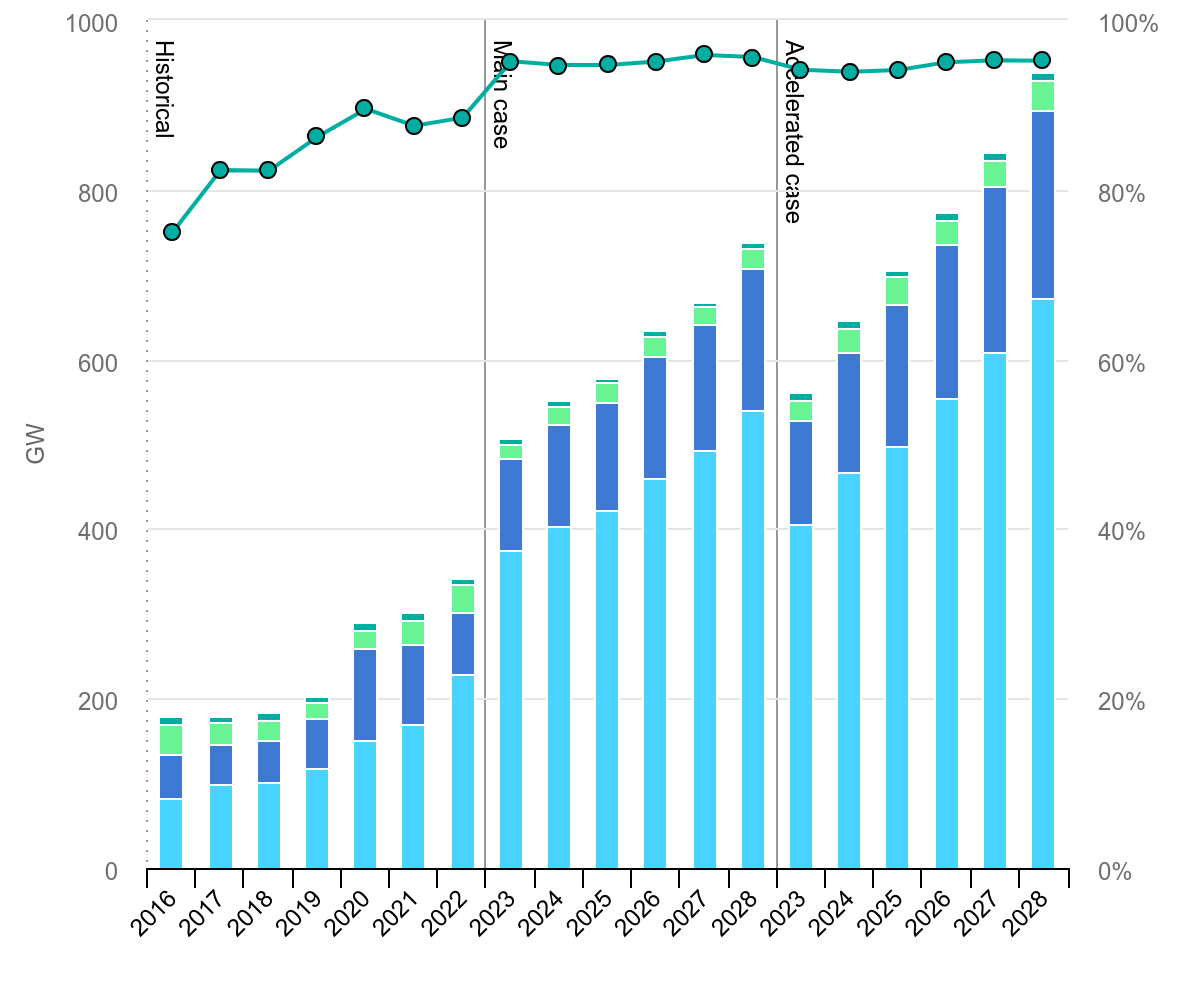
\includegraphics[width=0.9\columnwidth]{figure/rec_shares.png}
  \end{figure}
\end{column}
\begin{column}{0.5\columnwidth}
  Cumulative PV power capacity
  \begin{figure}
    \centering
    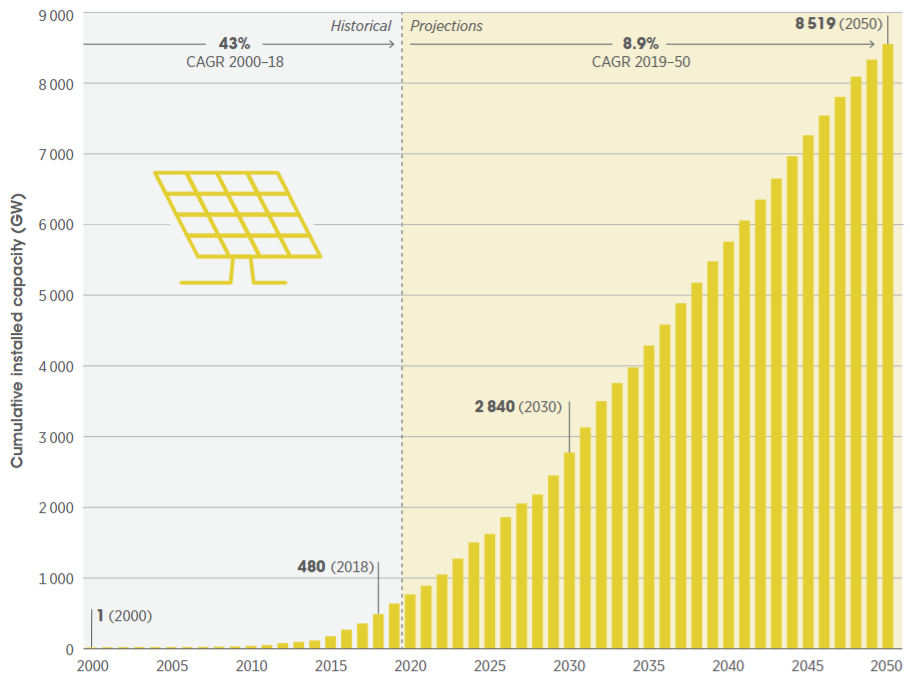
\includegraphics[width=0.9\columnwidth]{figure/pv_installation.png}
    \end{figure}
  \end{column}
\end{columns}

  {\tiny Source: \cite{irena2019}, \cite{iea2023}}
\end{frame}

\begin{frame}{PV plants classification}
  Traditionally we may identify two families of PV plants

  \textcolor{NTNUBlue}{Utility scale PV}: installed on dedicated locations, such as agricultural land. Their installed capacity may exceed 5 MW.

  \textcolor{NTNUBlue}{Distributed PV}: installed on existing structures, in the proximity of users. The installed capacity is between $\le$ 10 kW and 100 kW.

\end{frame}

\begin{frame}{PV plants classification: pros and cons}
  \begin{columns}
    \begin{column}{0.5\columnwidth}
      {\center \textcolor{NTNUBlue}{Utility scale}}\\
      \textcolor{NTNUgreen}{+} Cost effective: \$/MW half of rooftop installations\\
      \textcolor{NTNUgreen}{+} Extended life and reduced maintenance costs\\
      \textcolor{red}{-} Use of large land area\\
      \textcolor{red}{-} Degradation of wildlife habitat
    \end{column}
    \begin{column}{0.5\columnwidth}
      {\center \textcolor{NTNUBlue}{Distributed}}\\
      \textcolor{NTNUgreen}{+} Electricity is primary consumed by system owner, leading to lower cost for them\\
      \textcolor{NTNUgreen}{+} Reduced line losses\\
      \textcolor{red}{-} Limited space
    \end{column}
  \end{columns}
\end{frame}

\begin{frame}{Offshore PV (OPV)}
  Solve the problem of large scale PV system deployment without reducing land development. \\
  Furthermore: 
  \begin{itemize}
    \item reduce water evaporation
    \item water reduces temperature $\Rightarrow$ increase efficiency
    \item integration with Offshore Wind Turbine
  \end{itemize} 

  Nowadays the share of OPV is small, but the technology is relative young (first installation in 2007)
\end{frame}

\subsection{Mooring systems}
\begin{frame}{Mooring system}
  How can we ensure that the plant remains in a fixed position and is not tow away?

  Principal solutions:\\
  \textcolor{NTNUBlue}{MONOPILE} or \textcolor{NTNUBlue}{FLOATING}
  
\end{frame}

\begin{frame}{Mooring system - Pile}
  Suitable for shallow water depth less than 5 m (e.g. aquaculture ponds)\\
  In China projects for 1 GW installed capacity (8 km from shore)

  \begin{figure}
    \centering
    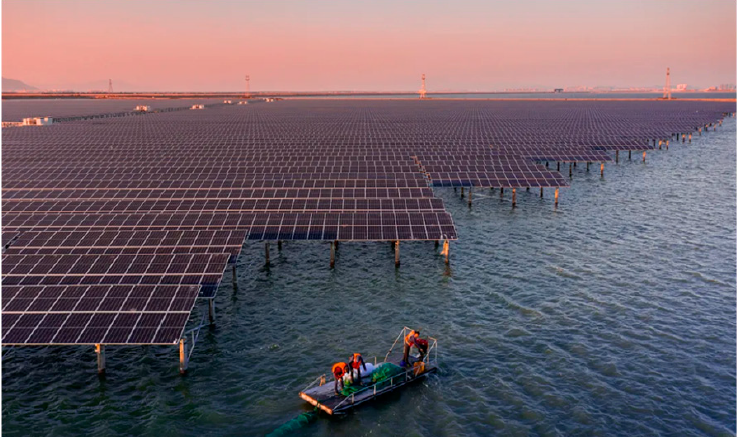
\includegraphics[width=0.3\columnwidth]{figure/floating_PV_china.png}
  \end{figure}

  \textcolor{NTNUgreen}{+} The mooring system offers stability\\
  \textcolor{NTNUgreen}{+} Reduction of water surface temp. $\Rightarrow$ Good for fish farming\\
  \textcolor{red}{-} Marine organism may attach and faster the pile corrosion\\
  \textcolor{red}{-} Need of transport of the piles

  {\tiny Figure source: \cite{jmse11112064}}
\end{frame}

\begin{frame}{Mooring system - Floating}
  \textcolor{NTNUBlue}{Idea:} The PV is mounted on a floating module whom movement is restricted through a multi-point mooring system 
  
  \textcolor{NTNUBlue}{Relatively young technology: }First installation in 2007

\end{frame}

\subsection{Types of floating structures}
\begin{frame}{Pontoon Floaters Module}
  \begin{figure}
    \centering
    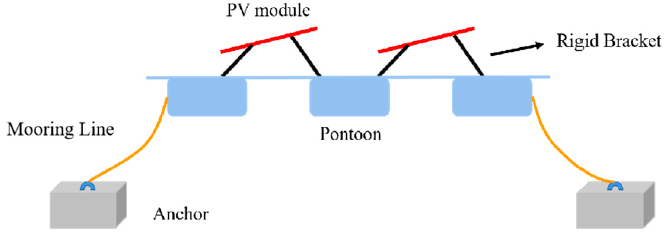
\includegraphics[width=0.4\columnwidth]{figure/pontoon.png}
  \end{figure}
  
  \textcolor{NTNUgreen}{+} Pontoons made of HDPE, which is resistant and recyclable\\
  \textcolor{NTNUgreen}{+} Easy installation\\
  \textcolor{NTNUgreen}{+} Covering water surface reduce evaporation\\
  \textcolor{NTNUgreen}{+} Cooling with water circulation and wind gusts effects\\
  \textcolor{red}{-} Interaction between floating bodies difficult to be modelled\\
  \textcolor{red}{-} Aquatic organism may attach the floating body and sink it

  {\tiny Figure source: \cite{jmse11112064}}
\end{frame}

\begin{frame}{Very Large Floating Structure}
  Floating module consists of a floating body and a flexible film on which PV are laid on.
  \begin{figure}
    \centering
    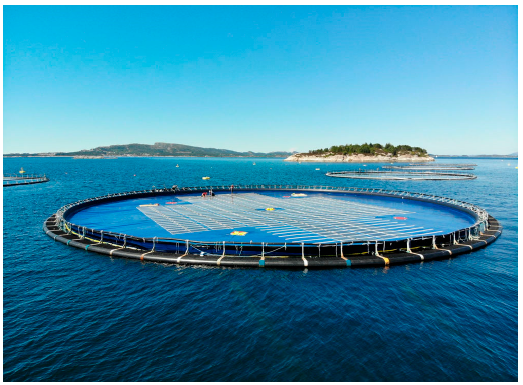
\includegraphics[width=0.3\columnwidth]{figure/vlfs.png}
  \end{figure}

  \textcolor{NTNUgreen}{+} Smaller air gap with water and better cooling effect\\
  \textcolor{NTNUgreen}{+} Flexible structure better accomplish wave action and so more suitable for offshore deployment\\
  \textcolor{red}{-} Single module is bulky and so difficult to install\\
  \textcolor{red}{-} Deep sea installation requires special mooring

  {\tiny Figure source: \cite{jmse11112064}}
\end{frame}

\begin{frame}{Very flexible floating structures (VFFS)}
  PV module are directly placed on the water's surface forming long structures (which can withstand large deflections).

  \begin{figure}
    \centering
    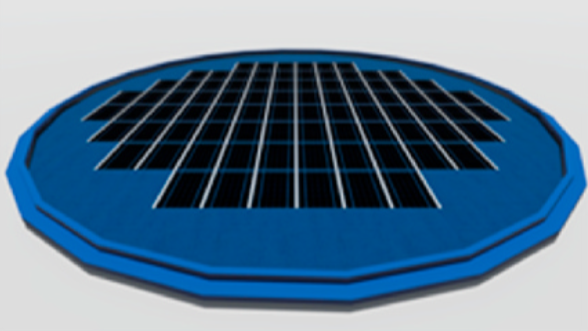
\includegraphics[width=0.3\columnwidth]{figure/vffs.png}
  \end{figure}

  \textcolor{NTNUgreen}{+} Excellent water-cooling effect\\
  \textcolor{NTNUgreen}{+} Reduced weight and simple mooring system\\
  \textcolor{NTNUgreen}{+} Reduce installation costs, possibility to tow ashore during winter\\
  \textcolor{red}{-} Earlier development stage

  {\tiny Figure source \cite{vffs_figure}}
\end{frame}

\subsection{Summary}
\begin{frame}{Conclusion}
  \textcolor{NTNUBlue}{Landscape utilization}: less consume of soil
  
  \textcolor{NTNUBlue}{Floating structure}: up to now mainly use of rigid structures, but nowadays also lightweight composite materials start to be used.

  \textcolor{NTNUBlue}{PV module}: development of the semiconductor technologies and improved efficiency for the lower temperature

  \textcolor{NTNUBlue}{Mooring system}: required increasing resistance for withstand the loads. Anti corrosion and anti biological parasites feature are important. 

  \textcolor{NTNUBlue}{Transportation and installation}: easier than with the use of monopiles.

\end{frame}

%   __  __      _        _          
%  |  \/  | ___| |_ _ __(_) ___ ___ 
%  | |\/| |/ _ \ __| '__| |/ __/ __|
%  | |  | |  __/ |_| |  | | (__\__ \
%  |_|  |_|\___|\__|_|  |_|\___|___/
                                  

\section{Quantification of the lost of inertia in the power system}
\begin{frame}{\insertsection}
  Increase of energy from renewable energy resources implies lost of inertia in the grid.
  \begin{figure}
    \centering
    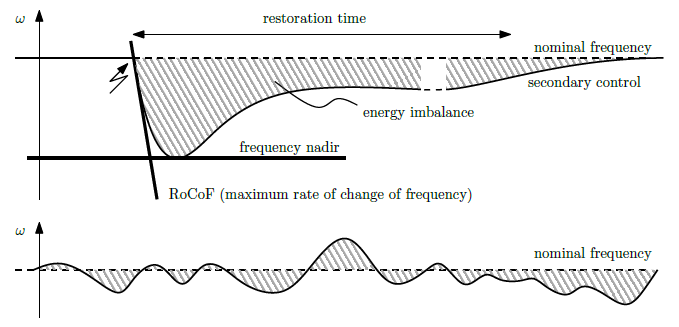
\includegraphics[width=0.5\columnwidth]{figure/frequency_disturbance.png}
  \end{figure} 
\end{frame}

\subsection{Metrics}
\begin{frame}{Time domain of the post-fault frequency evolution}{Classical metrics}
  \begin{itemize}[<+(1)->]
    \item Rate of Change of Frequency
    \begin{equation}
      \lvert \dot{\omega} \rvert _{max} = \max_i\left(\max_{t\ge0}\lvert \dot{\omega}_i(t) \rvert\right)
    \end{equation}
    
    \item Frequency Nadir
    \begin{equation}
      \lvert \underline{\omega} \rvert = \max_i\lvert\min_{t\ge0} \omega_i(t) \rvert
    \end{equation}
    \item Peak virtual inertia power injection
    \begin{equation}
      \bar{p}_v = \max_i\left(\max_{t\ge0}\lvert p_{v,i}(t) \rvert\right)
    \end{equation}
  \end{itemize}
\end{frame}

\begin{frame}
  Eigenvalue analysis
  \begin{itemize}
    \item Damping ratio of the power system
    \begin{equation}
      \zeta_{min} = \min_{k}\frac{-\sigma_k}{\sqrt{\sigma_k^2 + \omega_k^2}}
    \end{equation}
    with $\lambda_k=\sigma_k + \text{i}\omega_k$ the $k-th$ eigenvalue
  \end{itemize}
  
  Physical and virtual inertia of the devices
\begin{itemize}
  \item Total inertia
  \begin{equation}
    H_{total} = \sum_{i}H_i + \sum_{i} \tilde{H}_i = \sum_{i}\frac{m_i \omega_0}{2 S_{rated,i}} + \sum_{i} \frac{\tilde{m}_i \omega_0}{2 S_{rated,i}}
  \end{equation} 
\end{itemize}
\end{frame}

\begin{frame}{Time domain of the post-fault frequency evolution}{Energy metrics}
  \begin{itemize}[<+(1)->]
      \item Total energy imbalance
      \begin{equation}
        E_{\tau,\omega}=\int_{0}^{\tau}\sum_{i} q_i\omega_i^{2}dt=\int_{0}^{\tau} \omega^T Q \omega dt
      \end{equation}
      
      \item Total virtual inertia effort
      \begin{equation}
        E_{\tau,m}=\int_{0}^{\tau}\sum_{i} r_{m,i}p_{m,i}^{2}dt=\int_{0}^{\tau} p_{m}^T R_m p_{m} dt
      \end{equation}

      \item Total virtual damping effort
      \begin{equation}
        E_{\tau,d}=\int_{0}^{\tau}\sum_{i} r_{d,i}p_{d,i}^{2}dt=\int_{0}^{\tau} p_{d}^T R_d p_{d} dt
      \end{equation}
    \end{itemize}

    $q_i, r_m, and r_d$ are weights used for penalize one effort or the other
\end{frame}

\begin{frame}
  \begin{itemize}
    \item $\mathcal{H}_2$ norm: energy of the response to an impulse fault \textit{or} expected energy of the response to a white noise
    \begin{equation}
      \int_{0}^{\infty}\| y_p \|^2 dt = \int_{0}^{\infty} \omega^T Q \omega + p_{m}^T R_m p_{m} + p_{d}^T R_d p_{d} dt
    \end{equation}
    \textcolor{NTNUViolet}{
    Example: 
    \begin{gather}
      \text{System } \mathcal{G} :
      \begin{cases}
        \dot{x} = A x + G \eta \\
        y_p = C x
      \end{cases}
      \Rightarrow \| \mathcal{G} \|_2^2=\text{trace}\left(G^T P G\right)\\
      \text{Observability gramian: } PA + A^TP+C^TC=0
    \end{gather} 
    }
    \item $\mathcal{H}_{\infty }$ norm: root mean square gain from the disturbance to the performance output
  \end{itemize}
\end{frame}

\subsection{Example}
\begin{frame}{Use of the metrics}
  Test on the Kundor model with two different damping configuration
  \begin{columns}
    \begin{column}{0.5\columnwidth}
      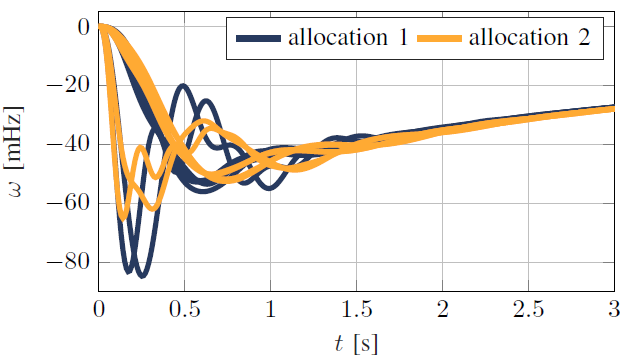
\includegraphics[width = \columnwidth]{figure/kundor_frequency.png}
    \end{column}
    \begin{column}{0.5\columnwidth}
      \begin{table}[h!]
        \centering
        \begin{tabular}{lcc}
        \toprule
        & Allocation 1 & Allocation 2 \\
        \midrule
        $H_{\text{total}}$ & 40.85 s & 40.85 s \\
        $\zeta_{\text{min}}$ & 0.1190 & 0.1206 \\
        $\left|\dot{\omega}\right|_{\max}$ & 0.8149 Hz/s & 0.8135 Hz/s \\
        $\left|\omega\right|$ & 84.8 mHz & 65.1 mHz \\
        $\mathcal{H}_2 $ & 1.5337 & 0.6522 \\
        $\mathcal{H}_{\infty} $ & 0.7454 & 0.2782 \\
        $\overline{P}_v$ & 118.38 MW & 7.0446 MW \\
        \bottomrule
        \end{tabular}
      
        \label{table:allocations}
        \end{table}
    \end{column}
  \end{columns}

  {\tiny Source: \cite{Increasing_the_Resilience}}
\end{frame}

% \section{PLL}  
% \begin{frame}{PLL schema}{\insertsection}
%   \begin{figure}
%     \tikzstyle{block} = [draw, fill=white!100, rounded corners]
\tikzstyle{sum_plus_nw} = [draw, fill=white, circle, label=above left:$+$]% sum with + in north west position
\tikzstyle{sum_minus_se} = [draw, fill=white, circle, label=below left:$-$]
\tikzstyle{input} = [coordinate]
\tikzstyle{output} = [coordinate]

\adjustbox{width=0.75\columnwidth, center}{
\begin{tikzpicture}[auto, >=latex']  
  \node [style = input] (v_abc) { $v_{abc}$}; % delta P input
  \node [style = block, right of = v_abc, node distance = 1.2cm] (PD) {PD};
  \node [style = sum_minus_se, right of = PD] (sum_P) {}; 

  \node [style = block, right of = sum_P] (LF) {LF};
  \node [style = block, right of = LF, node distance = 1.7cm] (VCO) {VCO};

  \node [style = output, right of = VCO] (fake_point) {};
  \node [style = output, below of = fake_point, node distance = 0.7cm] (fake_point2) {};
  \node [style = output, right of = fake_point, node distance = 0.5cm] (output) {};
  
  \draw [->] (v_abc) -> node[above] {$v_{abc}$} (PD);
  \draw [->] (PD) -> node[above] {$v_{q}$}  (sum_P);
  \draw [->] (sum_P) -> node[above] {$\epsilon_q$} (LF);
  \draw [->] (LF) -- node {$\Delta \hat{\omega}$} (VCO);
  \draw [-] (VCO) -- node {} (fake_point);
  \draw [->] (fake_point) -- node {$\hat{v}_{q}$} (output);
  \draw [-] (fake_point) -- node {} (fake_point2);
  \draw [->] (fake_point2) -| node {} (sum_P);
  
\end{tikzpicture}
} 
%   \end{figure}
% \begin{itemize}
%   \item Phase Detector \textcolor{NTNUBlue}{PD}
%   \item Loop Filter \textcolor{NTNUBlue}{LP}
%   \item Voltage Controlled Oscillator \textcolor{NTNUBlue}{VCO}
% \end{itemize}
% \end{frame}

% \begin{frame}{Phase Detector}{\insertsection}
%   \begin{figure}
%     \tikzstyle{block} = [draw, fill=white!100, rounded corners]
\tikzstyle{block_red} = [draw, color=red, fill=white!100, rounded corners]
\tikzstyle{sum_plus_nw} = [draw, fill=white, circle, label=above left:$+$]% sum with + in north west position
\tikzstyle{sum_minus_se} = [draw, fill=white, circle, label=below left:$-$]
\tikzstyle{input} = [coordinate]
\tikzstyle{output} = [coordinate]

\adjustbox{width=0.75\columnwidth, center}{
\begin{tikzpicture}[auto, >=latex']  
  \node [style = input] (v_abc) { $v_{abc}$}; % delta P input
  \node [style = block_red, right of = v_abc, node distance = 1.2cm] (PD) {PD};
  \node [style = sum_minus_se, right of = PD] (sum_P) {}; 

  \node [style = block, right of = sum_P] (LF) {LF};
  \node [style = block, right of = LF, node distance = 1.7cm] (VCO) {VCO};

  \node [style = output, right of = VCO] (fake_point) {};
  \node [style = output, below of = fake_point, node distance = 0.7cm] (fake_point2) {};
  \node [style = output, right of = fake_point, node distance = 0.5cm] (output) {};
  
  \draw [->] (v_abc) -> node[above] {$v_{abc}$} (PD);
  \draw [->] (PD) -> node[above] {$v_{q}$}  (sum_P);
  \draw [->] (sum_P) -> node[above] {$\epsilon_q$} (LF);
  \draw [->] (LF) -- node {$\Delta \hat{\omega}$} (VCO);
  \draw [-] (VCO) -- node {} (fake_point);
  \draw [->] (fake_point) -- node {$\hat{v}_{q}$} (output);
  \draw [-] (fake_point) -- node {} (fake_point2);
  \draw [->] (fake_point2) -| node {} (sum_P);
  
\end{tikzpicture}
} 
%   \end{figure}
%   Measures the $v_{abc}(t)$ voltage and \textcolor{NTNUBlue}{transforms} it in a $dq$ reference frame.
%   \begin{equation*}
%     abc \Rightarrow \alpha\beta \Rightarrow dq
%   \end{equation*}

%   Extracts the $v_q(t)$ component
% \end{frame}

% \begin{frame}{Loop Filter}{\insertsection}
%   \begin{figure}
%     \tikzstyle{block} = [draw, fill=white!100, rounded corners]
\tikzstyle{block_red} = [draw, color=red, fill=white!100, rounded corners]
\tikzstyle{sum_plus_nw} = [draw, fill=white, circle, label=above left:$+$]% sum with + in north west position
\tikzstyle{sum_minus_se} = [draw, fill=white, circle, label=below left:$-$]
\tikzstyle{input} = [coordinate]
\tikzstyle{output} = [coordinate]

\adjustbox{width=0.75\columnwidth, center}{
\begin{tikzpicture}[auto, >=latex']  
  \node [style = input] (v_abc) { $v_{abc}$}; % delta P input
  \node [style = block, right of = v_abc, node distance = 1.2cm] (PD) {PD};
  \node [style = sum_minus_se, right of = PD] (sum_P) {}; 

  \node [style = block_red, right of = sum_P] (LF) {LF};
  \node [style = block, right of = LF, node distance = 1.7cm] (VCO) {VCO};

  \node [style = output, right of = VCO] (fake_point) {};
  \node [style = output, below of = fake_point, node distance = 0.7cm] (fake_point2) {};
  \node [style = output, right of = fake_point, node distance = 0.5cm] (output) {};
  
  \draw [->] (v_abc) -> node[above] {$v_{abc}$} (PD);
  \draw [->] (PD) -> node[above] {$v_{q}$}  (sum_P);
  \draw [->] (sum_P) -> node[above] {$\epsilon_q$} (LF);
  \draw [->] (LF) -- node {$\Delta \hat{\omega}$} (VCO);
  \draw [-] (VCO) -- node {} (fake_point);
  \draw [->] (fake_point) -- node {$\hat{v}_{q}$} (output);
  \draw [-] (fake_point) -- node {} (fake_point2);
  \draw [->] (fake_point2) -| node {} (sum_P);
  
\end{tikzpicture}
} 
%   \end{figure}
%  Takes the error between the measured voltage $v_q$ and the estimated one $\hat{v}_q$ and computes the estimation of the frequency deviation at the bus connection $\Delta \hat{\omega}$
% \end{frame}

% \begin{frame}{Voltage-Controlled Oscillator}{\insertsection}
%   \begin{figure}
%     \tikzstyle{block} = [draw, fill=white!100, rounded corners]
\tikzstyle{block_red} = [draw, color=red, fill=white!100, rounded corners]
\tikzstyle{sum_plus_nw} = [draw, fill=white, circle, label=above left:$+$]% sum with + in north west position
\tikzstyle{sum_minus_se} = [draw, fill=white, circle, label=below left:$-$]
\tikzstyle{input} = [coordinate]
\tikzstyle{output} = [coordinate]

\adjustbox{width=0.75\columnwidth, center}{
\begin{tikzpicture}[auto, >=latex']  
  \node [style = input] (v_abc) { $v_{abc}$}; % delta P input
  \node [style = block, right of = v_abc, node distance = 1.2cm] (PD) {PD};
  \node [style = sum_minus_se, right of = PD] (sum_P) {}; 

  \node [style = block, right of = sum_P] (LF) {LF};
  \node [style = block_red, right of = LF, node distance = 1.7cm] (VCO) {VCO};

  \node [style = output, right of = VCO] (fake_point) {};
  \node [style = output, below of = fake_point, node distance = 0.7cm] (fake_point2) {};
  \node [style = output, right of = fake_point, node distance = 0.5cm] (output) {};
  
  \draw [->] (v_abc) -> node[above] {$v_{abc}$} (PD);
  \draw [->] (PD) -> node[above] {$v_{q}$}  (sum_P);
  \draw [->] (sum_P) -> node[above] {$\epsilon_q$} (LF);
  \draw [->] (LF) -- node {$\Delta \hat{\omega}$} (VCO);
  \draw [-] (VCO) -- node {} (fake_point);
  \draw [->] (fake_point) -- node {$\hat{v}_{q}$} (output);
  \draw [-] (fake_point) -- node {} (fake_point2);
  \draw [->] (fake_point2) -| node {} (sum_P);
  
\end{tikzpicture}
} 
%   \end{figure}
%  Takes the estimation of the frequency deviation at the bus connection $\Delta \hat{\omega}$  and estimates the voltage at the bus $\hat{v}_q$ 
% \end{frame}

\begin{frame}[allowframebreaks]

  \printbibliography
  
\end{frame}
      
\end{document}